\textbf{Ejemplo 1}
Hacer la gráfica de un gradiente aritmético de 6 ingresos anuales vencidos con primera cuota de   100.000COP.
\begin{itemize}
 \item a. Crecimiento de   250.000 COP
 \item b. Decreciente en   250.000 COP\\
\end{itemize}



\textbf{Solución:}

%La tabla ira centrada
\begin{center}
 \renewcommand{\arraystretch}{1.4}% Margenes de las celdas
 %Creación de la cuadricula de 3 columnas
 \begin{longtable}[H]{|c|c|c|}
  %Creamos una linea horizontal
  \hline
  %Definimos el color de la primera fila
  \rowcolor[HTML]{FFB183}
  %%%%% INICIO ASIGNACIÓN FECHA FOCAL %%%%%%%
  %%%%%%%%%% INICIO TITULO
  %Lo que se hace aquí es mezclar las 3 columnas en una sola
  \multicolumn{3}{|c|}{\cellcolor[HTML]{FFB183}\textbf{1. Asignación período focal}}                                                                    \\ \hline
  \multicolumn{3}{|c|}{No aplica}                                                                                                                     \\ \hline
  %%%%%%%%%% FIN TITULO
  %%%%% INICIO DECLARACIÓN DE VARIABLES %%%%%%%
  %%%%%%%%%% INICIO TITULO
  %Lo que se hace aquí es mezclar las 3 columnas en una sola
  \multicolumn{3}{|c|}{\cellcolor[HTML]{FFB183}\textbf{2. Declaración de variables}}                                                                  \\ \hline
  %%%%%%%%%% FIN TITULO
  %%%%%%%%%% INICIO DE MATEMÁTICAS
  %Cada & hace referencia al paso de la siguiente columna
  \multicolumn{2}{|c|}{\textbf{$\hspace{2.5 cm}\textit{Crecimiento}\hspace{2.5 cm}$}} & \textbf{$\hspace{2.5 cm}\textit{Decremiento}\hspace{2.5 cm}$} \\ \hline
  \multicolumn{2}{|c|}{$\hspace{2.5 cm}L=  250.000COP\hspace{2.5 cm}$}                        & $L=-  250.000?COP$                                                    \\
  \multicolumn{2}{|c|}{$\hspace{2.5 cm}n=6 \textit{naav}\hspace{2.5 cm}$}             & $n=6\textit{naav}$                                            \\ \hline
  
  
  %%%%%%%%%% FIN DE MATEMÁTICAS
  %%%%% FIN DECLARACIÓN DE VARIABLES
  
  
  %%%%% INICIO FLUJO DE CAJA
  \rowcolor[HTML]{FFB183}
  \multicolumn{3}{|c|}{\cellcolor[HTML]{FFB183}\textbf{3. Diagramas de los gradientes aritméticos}}                                                   \\ \hline
  %Mezclamos 3 columnas y pondremos el dibujo
  %%%%%%%%%%%%% INSERCIÓN DE LA IMAGEN
  %Deberán descargar las imágenes respectivas del drive y pegarlas en la carpeta
  %n_capitulo/img/ejemplos/1/capitulo1ejemplo1.pdf  (el /1/ es el numero del ejemplo)
  \multicolumn{3}{|c|}{ \includegraphics[trim=-5 -5 -5 -5 , scale=0.4]{6_Capitulo/ejemplos/1/Capitulo6Ejemplo1a.pdf} }                                \\
  
  \multicolumn{3}{|c|}{ \includegraphics[trim=-5 -5 -5 -5 , scale=0.4]{6_Capitulo/ejemplos/1/Capitulo6Ejemplo1b.pdf} }
  \\ \hline
  %%%%%%%%%%%%% FIN INSERCIÓN DE IMAGEN
  %%%%%FIN FLUJO DE CAJA
  
 \end{longtable}
 %Se crean dos lineas en blanco para que no quede el siguiente texto tan pegado
 %\newline \newline %USARLO SI CREES QUE ES NECESARIO
\end{center}
%%%%%%%%%%%%%%%%%%%%%%%%%%FIN EJERCICIO 3 %%%%%%%%%%%%%%%%%%%%%%%%%%%
